\documentclass[aspectratio=169,11pt]{beamer}

% ================================================================
% "TABIIY TILNI QAYTA ISHLASH" KURSI
% MA'RUZA 16 --- NLP amaliyotida MLOps (kursning YAKUNIY ma'ruzasi)
%              (d16_mlops.tex)
% Arxetiplar: [A][B][C][D][E] + 4 tsikl [F][G][H][I][J][K][L] +
%             [M][N][O][P][Q][R] + ilova [S]
% Rendered slayd soni: ~47 (kurs yakuni; L1-L15 chuqurligi)
% DIQQAT: QULFLANGAN [I] hand_example YO'Q (course_map hand_example: null);
%   keyingi P yo'q -> [I] slaydlar ILLYUSTRATIV, traceability izohsiz.
%   [Q] ko'prik = KAPSTONE HIMOYASI (keyingi P ga emas).
% ================================================================

% ================================================================
% RANGLAR  (asl fayldan o'zgarishsiz)
% ================================================================
\definecolor{cnublue}{rgb}{0.07,0.14,0.62}
\definecolor{cnubluelight}{rgb}{0.18,0.30,0.72}
\definecolor{cnubluebg}{rgb}{0.90,0.92,0.97}
\definecolor{deepblue}{rgb}{0.07,0.14,0.62}
\definecolor{deepred}{rgb}{0.60,0.00,0.00}
\definecolor{deepgreen}{rgb}{0.00,0.45,0.00}
\definecolor{halfgray}{gray}{0.55}

% ================================================================
% BEAMER MAVZU --- Boadilla + maxsus footer  (asl fayldan o'zgarishsiz)
% ================================================================
\usetheme{Boadilla}

\setbeamercolor{structure}{fg=cnublue}
\setbeamercolor{frametitle}{bg=cnublue,fg=white}
\setbeamercolor{title}{bg=cnublue,fg=white}
\setbeamercolor{block title}{bg=cnublue,fg=white}
\setbeamercolor{block body}{bg=cnubluebg,fg=black}
\setbeamercolor{alerted text}{fg=deepred}
\setbeamercolor{author in head/foot}{bg=cnubluelight,fg=white}
\setbeamercolor{section in head/foot}{bg=cnublue,fg=white}
\setbeamercolor{page number in head/foot}{bg=cnubluelight,fg=white}

\setbeamertemplate{mini frame}{}
\setbeamertemplate{mini frame in current section}{}
\setbeamertemplate{mini frame in current subsection}{}
\setbeamertemplate{headline}{}
\setbeamertemplate{navigation symbols}{}

\setbeamertemplate{footline}{%
  \leavevmode%
  \hbox{%
    \begin{beamercolorbox}[wd=0.17\paperwidth,ht=2.5ex,dp=1.25ex,leftskip=0.5em]{author in head/foot}%
      \usebeamerfont{author in head/foot}\scriptsize\insertshortauthor%
    \end{beamercolorbox}%
    \begin{beamercolorbox}[wd=0.69\paperwidth,ht=2.5ex,dp=1.25ex,center]{section in head/foot}%
      \usebeamerfont{section in head/foot}%
      \scriptsize\insertsectionnavigationhorizontal{0.69\paperwidth}{}{}%
    \end{beamercolorbox}%
    \begin{beamercolorbox}[wd=0.14\paperwidth,ht=2.5ex,dp=1.25ex,rightskip=0.5em]{page number in head/foot}%
      \hfill\scriptsize\color{white}%
      \insertframenumber{}/\inserttotalframenumber%
    \end{beamercolorbox}%
  }%
  \vskip0pt%
}

% ================================================================
% PAKETLAR  (asl fayldan o'zgarishsiz)
% ================================================================
\usepackage[utf8]{inputenc}
\usepackage[T1]{fontenc}
\usepackage{lmodern}
\usepackage{amsmath,amssymb}
\usepackage{booktabs}
\usepackage{xcolor}
\usepackage{listings}
\lstset{
    language=Python,
    basicstyle=\ttfamily\scriptsize,
    keywordstyle=\bfseries\color{deepblue},
    emphstyle=\ttfamily\color{deepred},
    stringstyle=\color{deepgreen},
    commentstyle=\itshape\color{halfgray},
    numbers=left,
    numberstyle=\scriptsize\color{halfgray},
    rulesepcolor=\color{cnublue!30},
    frame=shadowbox,
    breaklines=true,
    showstringspaces=false,
    tabsize=2
}
\usepackage{tcolorbox}
\tcbuselibrary{skins}
\tcbset{
  defbox/.style={colback=cnubluebg,colframe=cnublue,
                 fonttitle=\small\bfseries\color{white},
                 attach boxed title to top left={yshift=-2mm,xshift=4mm},
                 boxed title style={colback=cnublue,colframe=cnublue}},
  warnbox/.style={colback=orange!8,colframe=orange!70!black,
                  fonttitle=\small\bfseries},
  okbox/.style={colback=green!7,colframe=green!55!black,
                fonttitle=\small\bfseries}
}
\usepackage{tikz}
\usetikzlibrary{arrows.meta,positioning}

% ================================================================
% QO'SHIMCHALAR  (asl fayldan o'zgarishsiz)
% ================================================================
\AtBeginSection[]{%
  \begin{frame}{Prezentatsiya rejasi}
    \tableofcontents[currentsection]
  \end{frame}}

\newcommand{\bunda}[1]{{\small\textbf{bunda:}\; #1}}
\newcommand{\bajarildi}{{\color{deepgreen}\large$\checkmark$}\;}

% ================================================================
% METAMA'LUMOT
% ================================================================
\title[MLOps]{NLP amaliyotida MLOps}
\subtitle{Tabiiy tilni qayta ishlash --- 16-ma'ruza (yakuniy)}
\author[A.A.\,Abdulali]{A.A.\,Abdulali}
\date{10-iyul 2026}
\institute{11:00--12:20 \quad$\cdot$\quad mavzu \textnumero{}16}

% ================================================================
\begin{document}
% ================================================================

% ----------------------------------------------------------------
% [A] TITUL
% ----------------------------------------------------------------
\maketitle

% ================================================================
\section[Kirish]{Kirish: modeldan ishonchli xizmatga}
% ================================================================

% ----------------------------------------------------------------
% [B] TAKRORLASH: L15 va bugungi P15
% ----------------------------------------------------------------
\begin{frame}{Takrorlash: o'tgan darsdan ikki savol}
  \begin{columns}[T]
    \begin{column}{0.49\textwidth}
      \begin{tcolorbox}[warnbox,title=1-savol]
        \small
        L15/P15 da hujjat yordamchisi agentini quridik. U sizning
        noutbukingizda ishlaydi --- foydalanuvchilarga qanday yetkazamiz?
      \end{tcolorbox}
    \end{column}
    \begin{column}{0.49\textwidth}
      \begin{tcolorbox}[warnbox,title=2-savol]
        \small
        Model bir oydan keyin ham bir xil aniqlikda ishlaydimi? Yangi
        ma'lumot kelsa nima qilamiz?
      \end{tcolorbox}
    \end{column}
  \end{columns}
  \pause
  \vspace{4pt}
  \begin{columns}[T]
    \begin{column}{0.49\textwidth}
      \begin{tcolorbox}[okbox,title=1-javob]
        \small
        Modelni \textbf{xizmat} (API) qilib joylashtiramiz va
        \textbf{konteyner}ga (Docker) o'raymiz --- M4 da boshlagan ishimiz.
      \end{tcolorbox}
    \end{column}
    \begin{column}{0.49\textwidth}
      \begin{tcolorbox}[okbox,title=2-javob]
        \small
        Yo'q --- model \textbf{eskiradi} (drift). Monitoring, versiyalash va
        qayta o'qitish kerak. Bularning hammasi --- \textbf{MLOps}.
      \end{tcolorbox}
    \end{column}
  \end{columns}
\end{frame}

% ----------------------------------------------------------------
% [C] MAQSADLAR
% ----------------------------------------------------------------
\begin{frame}{Siz bugungi dars oxirida quyidagilarni bajara olasiz:}
  \begin{enumerate}\setlength\itemsep{6pt}
    \item \textbf{Tushuntira olasiz:} modelni ishlab chiqarishga uzatish
          bosqichlari (train $\to$ package $\to$ serve $\to$ monitor).
    \item \textbf{Tushuntira olasiz:} API yaratish va dokerlashtirish (FastAPI $+$ Docker).
    \item \textbf{Tushuntira olasiz:} model monitoringi, drift va versiyalash.
    \item \textbf{Tushuntira olasiz:} CI/CD payplayni va NLP loyihangizni davom
          ettirish yo'llari.
  \end{enumerate}
  \vspace{4pt}
  \begin{tcolorbox}[defbox,title=Oldindan talab]
    \footnotesize
    P15 (agent), M4 P16 (FastAPI/Docker). Tushuncha: API, JSON, model fayllari.
    Bu dars M4 da amalda qilganingizni \textbf{rasmiylashtiradi}.
  \end{tcolorbox}
\end{frame}

% ----------------------------------------------------------------
% [D] REJA
% ----------------------------------------------------------------
\begin{frame}{Bugungi dars rejasi:}
  \begin{center}
  \small
  \begin{tabular}{c p{5.2cm} c p{3.0cm}}
    \toprule
    \textbf{Tsikl}& \textbf{Mavzu} & \textbf{Vaqt} & \textbf{Asosiy g'oya}\\
    \midrule
    1 & Ishlab chiqarishga uzatish bosqichlari & 14 daq & train$\to$serve$\to$monitor \\
    2 & API va dokerlashtirish & 14 daq & FastAPI $+$ Docker \\
    3 & Monitoring va versiyalash & 14 daq & drift, model registry \\
    4 & CI/CD payplaynlari & 14 daq & test$\to$build$\to$deploy \\
    \midrule
      & Xulosa, kapstone himoyasi va keyingi yo'l & 14 daq & Kurs yakuni \\
    \bottomrule
  \end{tabular}
  \end{center}
  \vspace{4pt}
  \begin{tcolorbox}[warnbox,title=Bu dars --- kurs yakuni]
    \footnotesize\sloppy
    Kapstone "O'zbek hujjat yordamchisi" tayyor. Bugun uni ishonchli xizmatga
    aylantirish (MLOps) va himoya qilishni o'rganamiz.
  \end{tcolorbox}
\end{frame}

% ----------------------------------------------------------------
% [E] MUAMMO BIRINCHI
% ----------------------------------------------------------------
\begin{frame}{Bugungi dars uchun muammo: "menda ishlaydi" yetarli emas}
  \begin{columns}[T]
    \begin{column}{0.50\textwidth}
      \textbf{Notebook qayerda qiynaladi:}\\[3pt]
      \small
      \begin{tcolorbox}[warnbox,title={Faqat sizning muhitingiz},top=2pt,bottom=2pt]
        \footnotesize
        Model sizning Kaggle/noutbukingizda ishlaydi; boshqa kompyuterda
        kutubxona/versiya farqi tufayli ishlamasligi mumkin.
      \end{tcolorbox}
      \vspace{3pt}
      \begin{tcolorbox}[warnbox,title={Vaqt bilan eskiradi},top=2pt,bottom=2pt]
        \footnotesize
        Ma'lumot o'zgaradi (drift) $\Rightarrow$ aniqlik tushadi. Hech kim
        sezmasa, xizmat jimgina buziladi.
      \end{tcolorbox}
    \end{column}
    \begin{column}{0.46\textwidth}
      \textbf{Bugungi yechim (MLOps):}\\[4pt]
      \small
      \begin{enumerate}\setlength\itemsep{4pt}
        \item Modelni \textbf{paketlash} va \textbf{API} qilish.
        \item \textbf{Docker} bilan muhitni qotirib, hamma joyda bir xil ishlatish.
        \item \textbf{Monitoring} $+$ versiyalash $+$ \textbf{CI/CD} bilan
              avtomatlashtirish.
      \end{enumerate}
      \vspace{5pt}
      \begin{tcolorbox}[okbox,top=2pt,bottom=2pt]
        \footnotesize
        MLOps --- modelni ishonchli, takrorlanuvchi va yangilanuvchi xizmatga
        aylantirish amaliyoti.
      \end{tcolorbox}
    \end{column}
  \end{columns}
\end{frame}

% ================================================================
\section[Deploy]{Ishlab chiqarishga uzatish bosqichlari}
% ================================================================

% ----------------------------------------------------------------
% [F1] INTUITSIYA
% ----------------------------------------------------------------
\begin{frame}{Intuitsiya: oshxona retsepti emas, restoran}
  \begin{columns}[T]
    \begin{column}{0.52\textwidth}
      \small
      Notebook --- bu \textbf{retsept} (bir marta, o'zingiz uchun). Ishlab
      chiqarish --- bu \textbf{restoran}: ko'p mijoz, doimiy sifat, tezkor xizmat.\\[5pt]
      Yo'l: \textbf{o'qitish} $\to$ \textbf{paketlash} (model fayli) $\to$
      \textbf{serve} (API) $\to$ \textbf{monitoring} (sifatni kuzatish).
    \end{column}
    \begin{column}{0.44\textwidth}
      \begin{tcolorbox}[okbox,top=2pt,bottom=2pt]
        \footnotesize
        Modelni \texttt{save} qilib (m13 \texttt{save}, m14 \texttt{save\_index}),
        keyin yuklab xizmat qilamiz. O'qitish va xizmat --- alohida bosqichlar.
      \end{tcolorbox}
    \end{column}
  \end{columns}
\end{frame}

% ----------------------------------------------------------------
% [G1] RASMIY TA'RIF + BUNDA
% ----------------------------------------------------------------
\begin{frame}{Deploy bosqichlari: rasmiy ta'rif}
  \begin{tcolorbox}[defbox,title={Ta'rif: model hayot sikli}]
    \vspace{-0.4em}
    $$ \text{train} \rightarrow \text{package} \rightarrow \text{serve}
       \rightarrow \text{monitor} \rightarrow \text{(retrain)} $$
  \end{tcolorbox}
  \vspace{2pt}
  \bunda{train --- modelni o'qitish; package --- model fayli $+$ bog'liqliklarni
  to'plash; serve --- API orqali bashorat berish; monitor --- sifat va yukni
  kuzatish; retrain --- drift bo'lsa qayta o'qitish (sikl yopiladi).}
  \vspace{4pt}
  \footnotesize Asosiy g'oya: o'qitish bir marta, \textbf{serve} doimiy.
  Model artefakti (fayl) ikki bosqichni bog'laydi.
\end{frame}

% ----------------------------------------------------------------
% [H1] KELTIRIB CHIQARISH
% ----------------------------------------------------------------
\begin{frame}{Keltirib chiqarish: nega bosqichlarni ajratamiz?}
  \textbf{1-qadam.} O'qitish qimmat va kam --- har so'rovda qayta o'qitib bo'lmaydi.
  \pause
  \textbf{2-qadam.} O'qitilgan modelni \textbf{fayl}ga saqlaymiz (artefakt) ---
  bir marta o'qit, ko'p marta yukla.
  \pause
  \textbf{3-qadam.} Xizmat (serve) faqat faylni yuklab, bashorat beradi --- tez,
  arzon, masshtablanadigan.
  \pause
  \textbf{4-qadam.} Monitoring sifatni kuzatadi; pasaysa, retrain bosqichiga
  qaytadi (sikl).
  \begin{tcolorbox}[okbox,top=2pt,bottom=2pt]
    \small \textbf{Xulosa:} bosqichlarni ajratish --- tezlik, takrorlanuvchanlik
    va yangilanish imkonini beradi.
  \end{tcolorbox}
\end{frame}

% ----------------------------------------------------------------
% [I1] QO'LDA MISOL (ILLYUSTRATIV --- locked emas)
% ----------------------------------------------------------------
\begin{frame}{Qo'lda misol: yuklashni bir marta qilish}
  \begin{tcolorbox}[defbox,title={Ikki yondashuv}]
    \small Model fayli $400$ MB; yuklash $\approx 2$ s, bashorat $\approx 20$ ms.
  \end{tcolorbox}
  \vspace{0.2em}
  \begin{columns}[T]
    \begin{column}{0.54\textwidth}
      \footnotesize
      \textbf{Har so'rovda yuklash:} $2000 + 20 = 2020$ ms/so'rov --- juda sekin.\\[3pt]
      \textbf{Bir marta yuklash (startda):} har so'rov $\approx 20$ ms ---
      $\sim 100\times$ tezroq.
    \end{column}
    \begin{column}{0.42\textwidth}
      \begin{tcolorbox}[okbox,top=2pt,bottom=2pt]
        \footnotesize
        Shuning uchun model server \textbf{ishga tushganda bir marta} yuklanadi
        (global), so'rovlar uni qayta ishlatadi.
      \end{tcolorbox}
    \end{column}
  \end{columns}
\end{frame}

% ----------------------------------------------------------------
% [J1] SIZNING VAZIFANGIZ
% ----------------------------------------------------------------
\begin{frame}{Sizning vazifangiz: kunlik yuk}
  \begin{tcolorbox}[warnbox,title=Savol --- 60 soniya]
    \small
    Server bir marta yuklangan; har bashorat $20$ ms. Bir soniyada nechta so'rovni
    (taxminan, ketma-ket) bajara oladi?
  \end{tcolorbox}
  \pause
  \begin{tcolorbox}[okbox,title=Javob]
    \small
    $1000\ \text{ms} / 20\ \text{ms} = \mathbf{50}$ so'rov/soniya (bitta jarayon, ketma-ket).\\[3pt]
    \footnotesize Ko'proq kerak bo'lsa --- bir nechta nusxa (replica) yoki
    to'plamlab (batch) ishlash. Bu --- masshtablash.
  \end{tcolorbox}
\end{frame}

% ----------------------------------------------------------------
% [K1] KOD <-> FORMULA  [fragile]
% ----------------------------------------------------------------
\begin{frame}[fragile]{Kod $\leftrightarrow$ formula: modelni bir marta yuklash}
  \begin{columns}[T]
    \begin{column}{0.58\textwidth}
\begin{lstlisting}
# server ishga tushganda BIR MARTA (global)
clf = FineTunedClassifier()
clf.load("m13_model")          # package -> serve

def predict(text):             # har so'rov: faqat bashorat
    return clf.predict(text)
\end{lstlisting}
    \end{column}
    \begin{column}{0.38\textwidth}
      \textbf{Kod $\to$ bosqich:}\\[3pt]
      \footnotesize
      \begin{tabular}{p{1.7cm}p{2.0cm}}
        \toprule
        Kod & Bosqich \\
        \midrule
        \texttt{load} & package$\to$serve \\
        \texttt{predict} & serve \\
        \bottomrule
      \end{tabular}
      \vspace{4pt}
      \begin{tcolorbox}[okbox,top=2pt,bottom=2pt]
        \footnotesize
        \texttt{load} global (bir marta); \texttt{predict} har so'rovda.
        Bu --- M4 P16 dagi naqsh.
      \end{tcolorbox}
    \end{column}
  \end{columns}
\end{frame}

% ----------------------------------------------------------------
% [L1] TUZOG'
% ----------------------------------------------------------------
\begin{frame}{Deploy tuzog'i: train va serve muhitlari farqli}
  \begin{columns}[T]
    \begin{column}{0.52\textwidth}
      \begin{tcolorbox}[warnbox,title={Training-serving skew}]
        \small
        O'qitishda bir xil, serve da boshqa qayta ishlash (preprocessing)
        ishlatilsa, natija buziladi. Masalan tokenizator mos kelmasa.
      \end{tcolorbox}
    \end{column}
    \begin{column}{0.44\textwidth}
      \begin{tcolorbox}[okbox,top=2pt,bottom=2pt]
        \footnotesize
        \textbf{Yechim:} bir xil preprocessing kodi (m01) ikki bosqichda;
        model bilan birga saqlash/versiyalash.
      \end{tcolorbox}
    \end{column}
  \end{columns}
\end{frame}

% ================================================================
\section[API va Docker]{API yaratish va dokerlashtirish}
% ================================================================

% ----------------------------------------------------------------
% [F2] INTUITSIYA
% ----------------------------------------------------------------
\begin{frame}{Intuitsiya: modelni "rozetka"ga ulaymiz va qutiga solamiz}
  \begin{columns}[T]
    \begin{column}{0.52\textwidth}
      \small
      \textbf{API} --- modelga standart "rozetka": har kim HTTP so'rov yuborib
      javob oladi (til/qurilmadan mustaqil).\\[5pt]
      \textbf{Docker} --- modelni va uning butun muhitini bitta \textbf{qutiga}
      (konteyner) solish: hamma joyda aynan bir xil ishlaydi.
    \end{column}
    \begin{column}{0.44\textwidth}
      \begin{tcolorbox}[okbox,top=2pt,bottom=2pt]
        \footnotesize
        FastAPI (M4 P16) --- API; Docker --- muhitni qotiradi ("menda ishlaydi"
        muammosini yo'qotadi).
      \end{tcolorbox}
    \end{column}
  \end{columns}
\end{frame}

% ----------------------------------------------------------------
% [G2] RASMIY TA'RIF + BUNDA
% ----------------------------------------------------------------
\begin{frame}{API va konteyner: rasmiy ta'rif}
  \begin{tcolorbox}[defbox,title={Ta'rif: xizmat va konteyner}]
    \vspace{-0.4em}
    $$ \text{API}:\ \text{request} \rightarrow \text{model} \rightarrow \text{response};
       \qquad \text{image} = \text{base} + \text{deps} + \text{model} + \text{kod} $$
  \end{tcolorbox}
  \vspace{2pt}
  \bunda{API --- HTTP endpoint (masalan \texttt{POST /predict}); image --- Docker
  tasviri (base OS $+$ kutubxonalar $+$ model fayli $+$ ilova kodi); container ---
  image ning ishlayotgan nusxasi.}
  \vspace{4pt}
  \footnotesize Image bir marta quriladi, ko'p joyda bir xil ishga tushiriladi ---
  takrorlanuvchanlik kafolati.
\end{frame}

% ----------------------------------------------------------------
% [H2] KELTIRIB CHIQARISH
% ----------------------------------------------------------------
\begin{frame}{Keltirib chiqarish: nega Docker?}
  \textbf{1-qadam.} Model kutubxona versiyalariga bog'liq (torch, sklearn) ---
  boshqa kompyuterda farq qiladi.
  \pause
  \textbf{2-qadam.} Docker base OS $+$ aniq versiyalarni \textbf{qotiradi}
  (\texttt{requirements.txt}).
  \pause
  \textbf{3-qadam.} Image ichida model $+$ kod $+$ muhit --- bitta birlik.
  \pause
  \textbf{4-qadam.} Har joyda (bulut, server) \textbf{aynan} shu image ishga
  tushadi --- "menda ishlaydi" muammosi yo'qoladi.
  \begin{tcolorbox}[okbox,top=2pt,bottom=2pt]
    \small \textbf{Xulosa:} API --- kirish nuqtasi; Docker --- takrorlanuvchi muhit.
  \end{tcolorbox}
\end{frame}

% ----------------------------------------------------------------
% [I2] QO'LDA MISOL (ILLYUSTRATIV)
% ----------------------------------------------------------------
\begin{frame}{Qo'lda misol: Docker image qatlamlari}
  \begin{tcolorbox}[defbox,title={Image = qatlamlar yig'indisi}]
    \small base ($\approx 120$ MB) $+$ kutubxonalar ($\approx 800$ MB) $+$ model ($\approx 400$ MB).
  \end{tcolorbox}
  \vspace{0.2em}
  \begin{columns}[T]
    \begin{column}{0.54\textwidth}
      \footnotesize
      Jami image $\approx 1320$ MB. Kutubxona qatlami o'zgarmasa, qayta qurishda
      \textbf{keshlanadi} --- faqat o'zgargan qatlam qayta quriladi.
    \end{column}
    \begin{column}{0.42\textwidth}
      \begin{tcolorbox}[okbox,top=2pt,bottom=2pt]
        \footnotesize
        Shuning uchun \texttt{requirements} ni kod'dan oldin nusxalaymiz ---
        kesh samarali bo'ladi.
      \end{tcolorbox}
    \end{column}
  \end{columns}
\end{frame}

% ----------------------------------------------------------------
% [J2] SIZNING VAZIFANGIZ
% ----------------------------------------------------------------
\begin{frame}{Sizning vazifangiz: faqat kod o'zgardi}
  \begin{tcolorbox}[warnbox,title=Savol --- 60 soniya]
    \small
    Siz faqat ilova kodini o'zgartirdingiz (kutubxona va model o'sha). Qaysi
    qatlamlar keshdan olinadi, qaysi biri qayta quriladi?
  \end{tcolorbox}
  \pause
  \begin{tcolorbox}[okbox,title=Javob]
    \small
    base va kutubxona qatlamlari \textbf{keshdan} (o'zgarmagan); faqat
    \textbf{kod} qatlami qayta quriladi --- tez.\\[3pt]
    \footnotesize Shuning uchun \texttt{Dockerfile} da kam o'zgaradigan narsani
    (deps) yuqoriga, tez o'zgaradigan (kod) ni pastga qo'yamiz.
  \end{tcolorbox}
\end{frame}

% ----------------------------------------------------------------
% [K2] KOD <-> FORMULA  [fragile]
% ----------------------------------------------------------------
\begin{frame}[fragile]{Kod $\leftrightarrow$ bosqich: Dockerfile}
  \begin{columns}[T]
    \begin{column}{0.58\textwidth}
\begin{lstlisting}[language=bash]
FROM python:3.11-slim          # base
COPY requirements.txt .
RUN pip install -r requirements.txt  # deps (kesh)
COPY app.py model/ ./          # kod + model
EXPOSE 8000
CMD ["uvicorn", "app:app", "--host", "0.0.0.0"]
\end{lstlisting}
    \end{column}
    \begin{column}{0.38\textwidth}
      \textbf{Qator $\to$ qatlam:}\\[3pt]
      \footnotesize
      \begin{tabular}{p{1.7cm}p{2.0cm}}
        \toprule
        Qator & Qatlam \\
        \midrule
        \texttt{FROM} & base \\
        \texttt{RUN pip} & deps \\
        \texttt{COPY app} & kod \\
        \bottomrule
      \end{tabular}
      \vspace{4pt}
      \begin{tcolorbox}[okbox,top=2pt,bottom=2pt]
        \footnotesize
        deps kod'dan oldin --- kesh samarali. M4 P16 da shu Dockerfile.
      \end{tcolorbox}
    \end{column}
  \end{columns}
\end{frame}

% ----------------------------------------------------------------
% [L2] TUZOG'
% ----------------------------------------------------------------
\begin{frame}{Docker tuzog'i: ulkan image va sirlar}
  \begin{columns}[T]
    \begin{column}{0.52\textwidth}
      \begin{tcolorbox}[warnbox,title={Katta va xavfli image}]
        \small
        Keraksiz fayllar (datasets, keshlar) image ni shishiradi; API kalitlarini
        image ichiga yozish --- xavfsizlik xatosi.
      \end{tcolorbox}
    \end{column}
    \begin{column}{0.44\textwidth}
      \begin{tcolorbox}[okbox,top=2pt,bottom=2pt]
        \footnotesize
        \textbf{Yechim:} \texttt{.dockerignore}; slim base; sirlarni
        \textbf{environment} o'zgaruvchilari orqali (image ichida emas).
      \end{tcolorbox}
    \end{column}
  \end{columns}
\end{frame}

% ================================================================
\section[Monitoring]{Model monitoringi va versiyalash}
% ================================================================

% ----------------------------------------------------------------
% [F3] INTUITSIYA
% ----------------------------------------------------------------
\begin{frame}{Intuitsiya: model "qariydi", uni kuzatib turish kerak}
  \begin{columns}[T]
    \begin{column}{0.52\textwidth}
      \small
      Dunyo o'zgaradi: yangi so'zlar, yangi mavzular. Model o'sha eski
      ma'lumotda o'qitilgan $\Rightarrow$ aniqligi asta tushadi (\textbf{drift}).\\[5pt]
      Yechim: metrikalarni \textbf{kuzatish} (monitoring), pasaysa
      \textbf{ogohlantirish}, kerak bo'lsa yangi \textbf{versiya}ga o'tish.
    \end{column}
    \begin{column}{0.44\textwidth}
      \begin{tcolorbox}[okbox,top=2pt,bottom=2pt]
        \footnotesize
        Versiyalash: model registry da v1, v2, ... saqlanadi --- xato bo'lsa
        eski versiyaga \textbf{qaytish} (rollback) mumkin.
      \end{tcolorbox}
    \end{column}
  \end{columns}
\end{frame}

% ----------------------------------------------------------------
% [G3] RASMIY TA'RIF + BUNDA
% ----------------------------------------------------------------
\begin{frame}{Monitoring va drift: rasmiy ta'rif}
  \begin{tcolorbox}[defbox,title={Ta'rif: drift va ogohlantirish}]
    \vspace{-0.4em}
    $$ \Delta = M_{\text{baseline}} - M_{\text{joriy}}, \qquad
       \Delta > \tau \ \Rightarrow\ \text{ogohlantirish / retrain} $$
  \end{tcolorbox}
  \vspace{2pt}
  \bunda{$M_{\text{baseline}}$ --- dastlabki metrika (masalan F1); $M_{\text{joriy}}$
  --- joriy o'lchov; $\Delta$ --- pasayish; $\tau$ --- chegara (masalan $0.10$).}
  \vspace{4pt}
  \footnotesize Metrikalar yo'q bo'lsa (yorliqsiz), \textbf{data drift} ni
  kuzatamiz: kiruvchi matn taqsimoti o'zgardimi (yangi so'zlar ulushi).
\end{frame}

% ----------------------------------------------------------------
% [H3] KELTIRIB CHIQARISH
% ----------------------------------------------------------------
\begin{frame}{Keltirib chiqarish: drift ni qanday aniqlaymiz?}
  \textbf{1-qadam.} O'qitishdan keyin baseline metrikani qayd etamiz ($F1_0$).
  \pause
  \textbf{2-qadam.} Ishlab chiqarishda davriy ravishda joriy metrikani o'lchaymiz
  (yangi yorliqlangan namunada).
  \pause
  \textbf{3-qadam.} Farqni hisoblaymiz: $\Delta = F1_0 - F1_{\text{joriy}}$.
  \pause
  \textbf{4-qadam.} $\Delta$ chegaradan oshsa ($\tau$), ogohlantirish va qayta
  o'qitish (retrain) ishga tushadi.
  \begin{tcolorbox}[okbox,top=2pt,bottom=2pt]
    \small \textbf{Xulosa:} monitoring --- "jim buzilish"ni oldini oladi. Endi
    chegarani qo'lda ko'ramiz.
  \end{tcolorbox}
\end{frame}

% ----------------------------------------------------------------
% [I3] QO'LDA MISOL (ILLYUSTRATIV)
% ----------------------------------------------------------------
\begin{frame}{Qo'lda misol: drift chegarasi}
  \begin{tcolorbox}[defbox,title={Berilgan}]
    \small baseline $F1_0 = 0.85$; bir oydan keyin $F1_{\text{joriy}} = 0.70$;
    chegara $\tau = 0.10$.
  \end{tcolorbox}
  \vspace{0.2em}
  \begin{columns}[T]
    \begin{column}{0.54\textwidth}
      \textbf{Hisob:}
      \begin{align*}
        \Delta &= 0.85 - 0.70 = 0.15\\
        0.15 &> 0.10 = \tau \ \Rightarrow\ \textbf{retrain}
      \end{align*}
    \end{column}
    \begin{column}{0.42\textwidth}
      \begin{tcolorbox}[okbox,top=2pt,bottom=2pt]
        \footnotesize
        $\Delta=0.15$ chegaradan katta $\Rightarrow$ model eskirgan; yangi
        ma'lumotda qayta o'qitish kerak.
      \end{tcolorbox}
    \end{column}
  \end{columns}
\end{frame}

% ----------------------------------------------------------------
% [J3] SIZNING VAZIFANGIZ
% ----------------------------------------------------------------
\begin{frame}{Sizning vazifangiz: ogohlantirish kerakmi?}
  \begin{tcolorbox}[warnbox,title=Savol --- 60 soniya]
    \small
    baseline $F1_0 = 0.88$; joriy $F1 = 0.82$; chegara $\tau = 0.10$.\\[4pt]
    \textbf{$\Delta = ?$ \quad Ogohlantirish ishga tushadimi?}
  \end{tcolorbox}
  \pause
  \begin{tcolorbox}[okbox,title=Javob]
    \small
    $\Delta = 0.88 - 0.82 = 0.06 < 0.10$ $\Rightarrow$ \textbf{yo'q}, hozircha normal.\\[3pt]
    \footnotesize Pasayish bor, ammo chegaradan past --- kuzatishda davom etamiz.
    Chegara ($\tau$) ni juda past qo'ysak, behuda ogohlantirishlar ko'payadi.
  \end{tcolorbox}
\end{frame}

% ----------------------------------------------------------------
% [K3] KOD <-> FORMULA  [fragile]
% ----------------------------------------------------------------
\begin{frame}[fragile]{Kod $\leftrightarrow$ formula: drift tekshiruvi}
  \begin{columns}[T]
    \begin{column}{0.58\textwidth}
\begin{lstlisting}
BASELINE_F1 = 0.85
TAU = 0.10

def check_drift(current_f1):
    delta = BASELINE_F1 - current_f1
    if delta > TAU:
        return "retrain"      # ogohlantirish
    return "ok"

print(check_drift(0.70))      # retrain
\end{lstlisting}
    \end{column}
    \begin{column}{0.38\textwidth}
      \textbf{Kod $\to$ formula:}\\[3pt]
      \footnotesize
      \begin{tabular}{p{1.7cm}p{2.0cm}}
        \toprule
        Kod & Formula \\
        \midrule
        \texttt{delta} & $\Delta$ \\
        \texttt{> TAU} & $\Delta>\tau$ \\
        \bottomrule
      \end{tabular}
      \vspace{4pt}
      \begin{tcolorbox}[okbox,top=2pt,bottom=2pt]
        \footnotesize
        Davriy ish (cron) bu funksiyani chaqirib, drift bo'lsa retrain
        payplaynini boshlaydi.
      \end{tcolorbox}
    \end{column}
  \end{columns}
\end{frame}

% ----------------------------------------------------------------
% [L3] TUZOG'
% ----------------------------------------------------------------
\begin{frame}{Monitoring tuzog'i: versiyasiz model}
  \begin{columns}[T]
    \begin{column}{0.52\textwidth}
      \begin{tcolorbox}[warnbox,title={Rollback imkonsiz}]
        \small
        Yangi model yomon chiqsa va eski versiya saqlanmagan bo'lsa, ortga
        qaytib bo'lmaydi --- xizmat buzuq qoladi.
      \end{tcolorbox}
    \end{column}
    \begin{column}{0.44\textwidth}
      \begin{tcolorbox}[okbox,top=2pt,bottom=2pt]
        \footnotesize
        \textbf{Yechim:} model registry (v1, v2, ...) $+$ metadata; yomon
        versiyadan tezda \textbf{rollback}.
      \end{tcolorbox}
    \end{column}
  \end{columns}
\end{frame}

% ================================================================
\section[CI/CD]{CI/CD payplaynlari}
% ================================================================

% ----------------------------------------------------------------
% [F4] INTUITSIYA
% ----------------------------------------------------------------
\begin{frame}{Intuitsiya: konveyer --- qo'lda emas, avtomatik}
  \begin{columns}[T]
    \begin{column}{0.52\textwidth}
      \small
      Har o'zgarishda qo'lda test/qurish/joylash --- sekin va xatoga moyil.
      \textbf{CI/CD} buni \textbf{avtomatlashtiradi}: kod o'zgarsa, payplayn
      o'zi test qiladi, image quradi va joylaydi.\\[5pt]
      \textbf{CI} (integratsiya): test $+$ build. \textbf{CD} (yetkazish): deploy.
    \end{column}
    \begin{column}{0.44\textwidth}
      \begin{tcolorbox}[okbox,top=2pt,bottom=2pt]
        \footnotesize
        Bizning amaliyotlardagi \texttt{assert}lar --- CI testlarining asosi:
        ular avtomatik tekshiriladi.
      \end{tcolorbox}
    \end{column}
  \end{columns}
\end{frame}

% ----------------------------------------------------------------
% [G4] RASMIY TA'RIF + BUNDA
% ----------------------------------------------------------------
\begin{frame}{CI/CD: rasmiy ta'rif}
  \begin{tcolorbox}[defbox,title={Ta'rif: avtomatik payplayn}]
    \vspace{-0.4em}
    $$ \text{commit} \rightarrow \text{test} \rightarrow \text{build}
       \rightarrow \text{deploy} \quad (\text{har biri o'tsa, keyingisi}) $$
  \end{tcolorbox}
  \vspace{2pt}
  \bunda{commit --- kodni yuborish (git); test --- avtomatik tekshiruvlar
  (\texttt{assert}lar, unit testlar); build --- Docker image qurish; deploy ---
  yangi image ni serverga chiqarish. Bosqich yiqilsa, payplayn to'xtaydi.}
  \vspace{4pt}
  \footnotesize Maqsad: har o'zgarish ishonchli, takrorlanuvchi va tez yetkazilsin.
\end{frame}

% ----------------------------------------------------------------
% [H4] KELTIRIB CHIQARISH
% ----------------------------------------------------------------
\begin{frame}{Keltirib chiqarish: nega avtomatlashtirish?}
  \textbf{1-qadam.} Qo'lda test/deploy --- inson xatosi va sekinlik.
  \pause
  \textbf{2-qadam.} Har commit'da testlar \textbf{avtomatik} ishga tushadi ---
  buzuq kod erta ushlanadi.
  \pause
  \textbf{3-qadam.} Testlar o'tsa, image avtomatik quriladi (build).
  \pause
  \textbf{4-qadam.} Build o'tsa, avtomatik deploy --- tez va izchil yetkazish.
  \begin{tcolorbox}[okbox,top=2pt,bottom=2pt]
    \small \textbf{Xulosa:} CI/CD --- sifat darvozalarini avtomatlashtiradi.
    Kursdagi \texttt{assert}lar shu darvozalarning urug'i.
  \end{tcolorbox}
\end{frame}

% ----------------------------------------------------------------
% [I4] QO'LDA MISOL (ILLYUSTRATIV)
% ----------------------------------------------------------------
\begin{frame}{Qo'lda misol: payplayn bosqichlari}
  \begin{tcolorbox}[defbox,title={Payplayn: test -> build -> deploy}]
    \small Test $30$ s, build $90$ s, deploy $20$ s; ketma-ket.
  \end{tcolorbox}
  \vspace{0.2em}
  \begin{columns}[T]
    \begin{column}{0.54\textwidth}
      \footnotesize
      Jami $\approx 140$ s. Agar test yiqilsa, build va deploy
      \textbf{bajarilmaydi} --- buzuq kod ishlab chiqarishga chiqmaydi.
    \end{column}
    \begin{column}{0.42\textwidth}
      \begin{tcolorbox}[okbox,top=2pt,bottom=2pt]
        \footnotesize
        Tez fikr-mulohaza (feedback): xato bir-ikki daqiqada ma'lum bo'ladi,
        kunlar emas.
      \end{tcolorbox}
    \end{column}
  \end{columns}
\end{frame}

% ----------------------------------------------------------------
% [J4] SIZNING VAZIFANGIZ
% ----------------------------------------------------------------
\begin{frame}{Sizning vazifangiz: test yiqildi}
  \begin{tcolorbox}[warnbox,title=Savol --- 60 soniya]
    \small
    Payplaynda test bosqichi yiqildi (bitta \texttt{assert} o'tmadi). Keyin nima
    bo'ladi --- build va deploy bajariladimi?
  \end{tcolorbox}
  \pause
  \begin{tcolorbox}[okbox,title=Javob]
    \small
    \textbf{Yo'q} --- payplayn test bosqichida to'xtaydi; build/deploy
    bajarilmaydi. Buzuq kod ishlab chiqarishga chiqmaydi.\\[3pt]
    \footnotesize Shuning uchun ishonchli \texttt{assert}lar (kursdagidek) ---
    himoyaning birinchi darvozasi.
  \end{tcolorbox}
\end{frame}

% ----------------------------------------------------------------
% [K4] KOD <-> FORMULA  [fragile]
% ----------------------------------------------------------------
\begin{frame}[fragile]{Kod $\leftrightarrow$ bosqich: CI payplayn (yaml)}
  \begin{columns}[T]
    \begin{column}{0.58\textwidth}
\begin{lstlisting}[language=bash]
# .github/workflows/ci.yml (soddalashtirilgan)
on: [push]
jobs:
  pipeline:
    steps:
      - run: pytest            # test
      - run: docker build .    # build
      - run: ./deploy.sh       # deploy
\end{lstlisting}
    \end{column}
    \begin{column}{0.38\textwidth}
      \textbf{Qator $\to$ bosqich:}\\[3pt]
      \footnotesize
      \begin{tabular}{p{1.7cm}p{2.0cm}}
        \toprule
        Qator & Bosqich \\
        \midrule
        \texttt{pytest} & test \\
        \texttt{docker build} & build \\
        \texttt{deploy.sh} & deploy \\
        \bottomrule
      \end{tabular}
      \vspace{4pt}
      \begin{tcolorbox}[okbox,top=2pt,bottom=2pt]
        \footnotesize
        \texttt{push} bo'lsa avtomatik ishga tushadi; bosqich yiqilsa to'xtaydi.
      \end{tcolorbox}
    \end{column}
  \end{columns}
\end{frame}

% ----------------------------------------------------------------
% [L4] TUZOG'
% ----------------------------------------------------------------
\begin{frame}{CI/CD tuzog'i: testsiz payplayn}
  \begin{columns}[T]
    \begin{column}{0.52\textwidth}
      \begin{tcolorbox}[warnbox,title={Faqat deploy avtomatik}]
        \small
        Testsiz "avtomatik deploy" --- buzuq kodni tezroq ishlab chiqarishga
        chiqaradi. Avtomatlashtirish testsiz xavfli.
      \end{tcolorbox}
    \end{column}
    \begin{column}{0.44\textwidth}
      \begin{tcolorbox}[okbox,top=2pt,bottom=2pt]
        \footnotesize
        \textbf{Yechim:} deploy'dan oldin majburiy test darvozasi; nazorat
        sinovlari (smoke test) deploy'dan keyin.
      \end{tcolorbox}
    \end{column}
  \end{columns}
\end{frame}

% ================================================================
\section[Xulosa]{Xulosa, kapstone himoyasi va keyingi yo'l}
% ================================================================

% ----------------------------------------------------------------
% [M] O'ZBEK TILIGA XOSLIK (majburiy arxetip)
% ----------------------------------------------------------------
\begin{frame}{O'zbek tilida: NLP ekotizimi va ochiq muammolar}
  \begin{columns}[T]
    \begin{column}{0.50\textwidth}
      \textbf{1. Mavjud resurslar:}\\[3pt]
      \small
      Ochiq modellar paydo bo'lmoqda: UzBERT, Tahrirchi modellari va boshqalar.
      Ammo ingliz tiliga nisbatan resurslar hamon kam.
      \begin{tcolorbox}[warnbox,title=Ochiq muammolar,top=2pt,bottom=2pt]
        \footnotesize
        Yorliqlangan ma'lumot kamligi; ishonchli morfologik tahlilchi;
        domenga xos (huquq, tibbiyot) modellar.
      \end{tcolorbox}
    \end{column}
    \begin{column}{0.46\textwidth}
      \textbf{2. Sizning hissangiz:}\\[3pt]
      \small
      Kursda qurgan modullaringiz --- haqiqiy hissaning boshlanishi.
      \begin{tcolorbox}[okbox,top=2pt,bottom=2pt]
        \footnotesize
        Yo'nalishlar: o'zbek korpus/benchmark yaratish; ochiq model fine-tune
        qilib ulashish; domenga xos yordamchilar qurish.
      \end{tcolorbox}
    \end{column}
  \end{columns}
\end{frame}

% ----------------------------------------------------------------
% [N] SINTEZ
% ----------------------------------------------------------------
\begin{frame}{Sintez: notebook va ishlab chiqarish}
  \begin{center}\small
  \begin{tabular}{p{3.2cm}p{3.6cm}p{4.0cm}}
    \toprule
    \textbf{Jihat} & \textbf{Notebook (tadqiqot)} & \textbf{Ishlab chiqarish (MLOps)} \\
    \midrule
    Maqsad & sinash, o'rganish & ishonchli xizmat \\
    Muhit & shaxsiy & Docker (qotirilgan) \\
    Sifat & bir martalik & monitoring $+$ drift \\
    Yangilash & qo'lda & CI/CD $+$ versiyalash \\
    \bottomrule
  \end{tabular}
  \end{center}
  \vspace{4pt}
  \begin{tcolorbox}[okbox,title=Asosiy g'oya,top=2pt,bottom=2pt]
    \footnotesize
    MLOps modelni \textbf{ishonchli, takrorlanuvchi, yangilanuvchi} xizmatga
    aylantiradi: train$\to$package$\to$serve$\to$monitor, Docker, registry, CI/CD.
  \end{tcolorbox}
\end{frame}

% ----------------------------------------------------------------
% [O] SEMINAL MANBA + MUHOKAMA SAVOLI
% ----------------------------------------------------------------
\begin{frame}{Seminal manba: Sculley va boshqalar (2015)}
  \begin{tcolorbox}[defbox,title=Manba]
    \small
    Sculley, D., va boshq.\ (2015). \textbf{Hidden Technical Debt in Machine
    Learning Systems.} \textit{NeurIPS 28.}
  \end{tcolorbox}
  \vspace{5pt}
  \textbf{Ahamiyati:}
  \begin{itemize}\small\setlength\itemsep{3pt}
    \item Model kodi --- ML tizimining kichik qismi; atrofidagi infratuzilma katta.
    \item "Yashirin texnik qarz": monitoringsiz model jimgina eskiradi.
    \item MLOps amaliyotining nazariy asosi bo'ldi.
  \end{itemize}
  \vspace{5pt}
  \begin{tcolorbox}[warnbox,title=Muhokama savoli]
    \small
    O'zbek tilidagi xizmat uchun qaysi "yashirin qarz" eng xavfli --- drift,
    yorliqlangan ma'lumot kamligi, yoki tokenizator nomuvofiqligi? Nega?
  \end{tcolorbox}
\end{frame}

% ----------------------------------------------------------------
% [P] MAQSADLAR BAJARILDI
% ----------------------------------------------------------------
\begin{frame}{Bugungi maqsadlar bajarildi}
  \begin{enumerate}\setlength\itemsep{7pt}
    \item \bajarildi \textbf{Tushuntirdik:} deploy bosqichlari
          (train$\to$package$\to$serve$\to$monitor).
    \item \bajarildi \textbf{Tushuntirdik:} API (FastAPI) va dokerlashtirish (Docker).
    \item \bajarildi \textbf{Tushuntirdik:} monitoring, drift ($\Delta>\tau$) va versiyalash.
    \item \bajarildi \textbf{Tushuntirdik:} CI/CD payplayni va o'zbek NLP da
          keyingi yo'l.
  \end{enumerate}
\end{frame}

% ----------------------------------------------------------------
% [Q] KO'PRIK: KAPSTONE HIMOYASI (keyingi P ga emas --- kurs yakuni)
% ----------------------------------------------------------------
\begin{frame}{Kapstone himoyasi: "O'zbek hujjat yordamchisi"}
  \begin{center}
  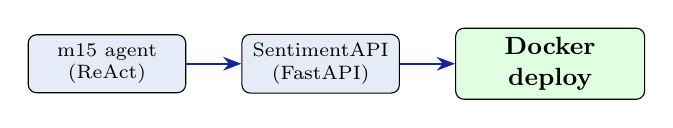
\begin{tikzpicture}[
      mod/.style={draw, fill=cnubluebg, rounded corners=3pt,
                  minimum width=2.0cm, minimum height=0.7cm,
                  font=\scriptsize, align=center},
      fin/.style={draw, fill=green!12, rounded corners=3pt,
                  minimum width=2.4cm, minimum height=0.7cm,
                  font=\small\bfseries, align=center},
      arr/.style={-{Stealth}, thick, color=cnublue}
  ]
    \node[mod] (m15) {m15 agent\\ (ReAct)};
    \node[mod, right=0.7cm of m15] (api) {SentimentAPI\\ (FastAPI)};
    \node[fin, right=0.7cm of api] (dep) {Docker\\ deploy};
    \draw[arr] (m15)--(api); \draw[arr] (api)--(dep);
  \end{tikzpicture}
  \end{center}
  \vspace{4pt}
  \begin{columns}[T]
    \begin{column}{0.52\textwidth}
      \textbf{Himoyada ko'rsating:}\\[3pt]
      \small
      \begin{itemize}\setlength\itemsep{2pt}
        \item \texttt{m15 DocumentAssistantAgent} jonli demo (o'zbekcha so'rov).
        \item \texttt{SentimentAPI} (FastAPI) --- \texttt{POST /predict}.
        \item Docker bilan ishga tushirish (M4 P16).
      \end{itemize}
    \end{column}
    \begin{column}{0.44\textwidth}
      \begin{tcolorbox}[okbox,title=Tayyorlab keling,top=2pt,bottom=2pt]
        \footnotesize
        16 kun mehnatingiz --- bitta ishlaydigan tizim. Modullar (m01--m15),
        API va MLOps tushunchalarini bog'lab tushuntiring.
      \end{tcolorbox}
    \end{column}
  \end{columns}
\end{frame}

% ----------------------------------------------------------------
% [R] ADABIYOTLAR + KURS YAKUNI
% ----------------------------------------------------------------
\begin{frame}{Adabiyotlar va kurs yakuni}
  \begin{enumerate}\small\setlength\itemsep{4pt}
    \item Sculley, D., va boshq.\ (2015). \textit{Hidden Technical Debt in ML Systems.} NeurIPS 28.
    \item Huyen, C.\ (2022). \textit{Designing Machine Learning Systems.} O'Reilly.
    \item \texttt{fastapi.tiangolo.com} va \texttt{docs.docker.com} --- API va konteyner.
    \item Google / Microsoft MLOps qo'llanmalari (monitoring, CI/CD).
  \end{enumerate}
  \vspace{4pt}
  \begin{tcolorbox}[okbox,title=Tabriklaymiz!,top=2pt,bottom=2pt]
    \footnotesize
    16 kunda klassik NLP'dan zamonaviy agentlargacha bordingiz va ishlaydigan
    o'zbek tili yordamchisini qurdingiz. Endi --- bu bilimni real loyihalarda
    qo'llang va o'zbek NLP ekotizimiga hissa qo'shing.
  \end{tcolorbox}
\end{frame}

% ================================================================
% [S] ILOVALAR (appendix --- slayd soniga kirmaydi)
% ================================================================
\appendix

\begin{frame}{Ilova S1: model registry va A/B test}
  \small
  \textbf{Model registry} --- model versiyalari ombori (v1, v2, ...) metadata bilan
  (metrika, sana, ma'lumot). Imkonlar:
  \begin{itemize}\setlength\itemsep{2pt}
    \item Rollback --- yomon versiyadan eskisiga qaytish.
    \item A/B test --- yangi (v2) va eski (v1) modelni real trafikda solishtirish.
  \end{itemize}
  \bunda{A/B test: trafikning bir qismi v2 ga yo'naltiriladi; metrikalar
  solishtiriladi; v2 yaxshi bo'lsa to'liq o'tkaziladi.}
\end{frame}

\begin{frame}[fragile]{Ilova S2: smoke test (deploy'dan keyin)}
  \small
  Deploy'dan keyin xizmat haqiqatan ishlayotganini tez tekshiramiz:
\begin{lstlisting}[language=bash]
curl -X POST localhost:8000/predict \
     -d '{"text": "mahsulot zo'r"}'
# kutilgan: {"sentiment": "ijobiy", "confidence": ...}
\end{lstlisting}
  \bunda{smoke test --- eng muhim yo'lning ishlashini tasdiqlovchi minimal
  sinov; CI/CD da deploy bosqichidan keyin avtomatik bajariladi.}
\end{frame}

\end{document}
